%; whizzy paragraph -pdf xpdf -latex ./whizzypdfptex.sh
%; whizzy-paragraph "^\\\\begin{frame}\\|\\\\emtext"
% latex beamer presentation.
% platex, latex-beamer でコンパイルすることを想定。 

%     Tokyo Debian Meeting resources
%     Copyright (C) 2012 Junichi Uekawa

%     This program is free software; you can redistribute it and/or modify
%     it under the terms of the GNU General Public License as published by
%     the Free Software Foundation; either version 2 of the License, or
%     (at your option) any later version.

%     This program is distributed in the hope that it will be useful,
%     but WITHOUT ANY WARRANTY; without even the implied warreanty of
%     MERCHANTABILITY or FITNESS FOR A PARTICULAR PURPOSE.  See the
%     GNU General Public License for more details.

%     You should have received a copy of the GNU General Public License
%     along with this program; if not, write to the Free Software
%     Foundation, Inc., 51 Franklin St, Fifth Floor, Boston, MA  02110-1301 USA

\documentclass[cjk,dvipdfmx,12pt]{beamer}
\usetheme{Tokyo}
\usepackage{monthlypresentation}

%  preview (shell-command (concat "evince " (replace-regexp-in-string "tex$" "pdf"(buffer-file-name)) "&")) 
%  presentation (shell-command (concat "xpdf -fullscreen " (replace-regexp-in-string "tex$" "pdf"(buffer-file-name)) "&"))
%  presentation (shell-command (concat "evince " (replace-regexp-in-string "tex$" "pdf"(buffer-file-name)) "&"))

%http://www.naney.org/diki/dk/hyperref.html
%日本語EUC系環境の時
\AtBeginDvi{\special{pdf:tounicode EUC-UCS2}}
%シフトJIS系環境の時
%\AtBeginDvi{\special{pdf:tounicode 90ms-RKSJ-UCS2}}

\newenvironment{commandlinesmall}%
{\VerbatimEnvironment
  \begin{Sbox}\begin{minipage}{1.0\hsize}\begin{fontsize}{8}{8} \begin{BVerbatim}}%
{\end{BVerbatim}\end{fontsize}\end{minipage}\end{Sbox}
  \setlength{\fboxsep}{8pt}
% start on a new paragraph

\vspace{6pt}% skip before
\fcolorbox{dancerdarkblue}{dancerlightblue}{\TheSbox}

\vspace{6pt}% skip after
}
%end of commandlinesmall

\title{東京エリアDebian勉強会}
\subtitle{第117回 2014年9月度}
\author{野島貴英}
\date{2014年9月27日}
\logo{
\includegraphics[width=8cm]{image200607/openlogo-light.eps}}

\begin{document}

\begin{frame}
\titlepage{}
\end{frame}

\begin{frame}{設営準備にご協力ください。}
会場設営よろしくおねがいします。
\end{frame}

\begin{frame}{Agenda}
 \begin{minipage}[t]{0.45\hsize}
  \begin{itemize}
   \item 注意事項
	 \begin{itemize}
	  \item 写真はセミナールーム内のみ可です。
          \item 出入りは自由でないので、もし外出したい方は、野島まで一声くださいませ。
	 \end{itemize}
   \item 事前課題発表
  \end{itemize}
 \end{minipage} 
 \begin{minipage}[t]{0.45\hsize}
  \begin{itemize}
   \item 最近あったDebian関連のイベント報告
	 \begin{itemize}
	  \item 第116回 東京エリアDebian勉強会
	 \end{itemize}
   \item Debian Trivia Quiz
   \item DebConf14のビデオ紹介
   \item 今後のイベント
   \item 今日の宴会場所
  \end{itemize}
 \end{minipage}
\end{frame}

\section{事前課題}
\emtext{事前課題}
{\footnotesize
\begin{prework}{ 野島 }
 xmrisのパッケージ化作業を続ける。
\end{prework}

\begin{prework}{ roger\@localet.com }
お世話になります。Roger です。
初めてなので、特に課題がなし、見学だけをさせていただきます。
宜しくお願い致します。
\end{prework}

\begin{prework}{ dictoss(杉本 典充) }

\begin{itemize}
\item ITP中のwx3.0-docパッケージの修正、パッケージメンテナチームへメールを送る
\item Debian 新メンテナーガイドを読んで理解する
\end{itemize}

\end{prework}

\begin{prework}{ 吉野(yy\_{}y\_{}ja\_{}jp) }

DDTSS\footnote{\url{http://ddtp.debian.net/ddtss/index.cgi/ja}}

\end{prework}

\begin{prework}{ henrich }

\begin{itemize}
\item net-snmpパッケージのバグレポートを眺める
\item debianjpでの改善案を練る
\end{itemize}

\end{prework}

\begin{prework}{ 野首(\@knok) }
\begin{itemize}
\item groongaのドキュメント整備
\item jessieインストーラの調査
\item libsixelのパッケージ化 \\
\url{https://github.com/saitoha/libsixel}
\end{itemize}
\end{prework}


}

\section{イベント報告}
\emtext{イベント報告}

\begin{frame}{第116回東京エリアDebian勉強会}
 
\begin{itemize}
\item 場所はスクウェア・エニックスさんのセミナルームをお借りしての開催でした。
\item なかおさんにより、ISAC tokyo 2014にも出展した内容でもある件についてお話がありました。タイルマップサーバーをDebianで作り、JAXAの海面温度データをOpenStreetMapに重ねるという内容でした。
\item zinraiさんによるDebianでのAnsibleの話題についてのBOFが行われました。
\item 残りの時間はもくもく会を行い、最後に成果発表をしました。
\end{itemize} 

\end{frame}

\section{Debian Trivia Quiz}
\emtext{Debian Trivia Quiz}
\begin{frame}{Debian Trivia Quiz}

  Debian の常識、もちろん知ってますよね?
知らないなんて恥ずかしくて、知らないとは言えないあんなことやこんなこと、
みんなで確認してみましょう。

今回の出題範囲は\url{debian-devel-announce@lists.debian.org},
\url{debian-news@lists.debian.org} に投稿された
内容などからです。

\end{frame}

\subsection{問題}

%; whizzy-master ../debianmeetingresume201311.tex
% 以上の設定をしているため、このファイルで M-x whizzytex すると、whizzytexが利用できます。
%

\santaku
{FSFがDebian Projectへ案内をしてきた、自由ソフトウェアのみの元で動かすことの出来るハードウェアについてのデータベースは次のうちどれ?}
{h-node.org}
{wiki.debian.org/Hardware}
{openbenchmarking.org}
{A}
{日本語の本件のニュースはsourceforge.jpの記事参照:http://sourceforge.jp/magazine/14/09/11/062900 。FSFはmainリポジトリのみのパッケージで構成されるDebianは自由ソフトウェアとみているとのこと。}

\santaku
{Debconf14の参加人数は結局何人?}
{900人}
{300人}
{1000人}
{B}
{300人とのことです。参考:Debconf13は290人、Debconf12は176人、Debconf11は335人でした。}

\santaku
{8/17にbuilddにて使われるアーカイブがどこからもアクセスできるようになりました。urlはどれ?}
{ftp.debian.or.jp/debian/}
{ftp.jp.debian.org/debian/}
{incoming.debian.org/debian-buildd/}
{C}
{今までは、どこからもアクセスできたわけではなかったようです。}

\santaku
{2014/8/19に登録商標としてDebianロゴが正式に登録されたそうです。どこの国の登録商標でしょうか?}
{米国}
{日本}
{スイス}
{A}
{United States Patent and Trademark Officeになります(つまり米国。)登録されたDebianロゴのデザインは http://tdr.uspto.gov/search.action?sn=86037470 からたどると閲覧できます。}

\santaku
{2014/8/24のBitFromDPLによれば、Debian Projectは仮想通貨による寄付をはじめて受け付けたそうです。具体的には何という仮想通貨でしょう?}
{Greeコイン}
{Crysta}
{BitCoin}
{C}
{Debian ProjectはBitCoinをそのまま受け付けることが出来るシステムを持たないため、その場限りの方法で受け取ったとのことです。今後、こういった仮想通貨での寄付の受け取りと取り扱いについて意見がほしいとのことです。}

\santaku
{検索エンジンのDuckDuckGOより、収入が入ったとのことです。2014/8/24現在、月当たりのDuckDuckGOからの平均収入は月額いくらでしょう?}
{\$10}
{\$152}
{\$1400}
{B}
{Debianパッケージに含まれるブラウザにデフォルトで登録されている検索エンジンの候補としてDuckDuckGOが搭載されていることによる収入となります。DuckDuckGOはプライバシーに配慮した検索エンジンです。最近は、iphone のsafariブラウザにあらかじめ登録される検索エンジンの候補としても上がり有名になりつつあります。URLはhttps://duckduckgo.com/}

\santaku
{2014/8/27にDebian archiveに搭載された2つの新しいアーキテクチャは、arm64以外には以下のどれ?}
{sparc}
{mips}
{ppc64el}
{C}
{ 64 bit powerpcのlittle endianモードのポーティングとのことです。すでに存在するppc64はbig endianのバイナリのポートティングとなります。}

\santaku
{2014/8/31にて、arm64ポートのDebian開発用に、無償のARM64用のコンパイラ・デバッガ等の開発キットの提供が行われたようです。製品名は以下のどれ?}
{Microsoft Visual Studio}
{IAR Embedded Workbench}
{DS-5 Development Studio}
{C}
{ Debian Editionとのことです。アナウンスによれば、ダウンロードリンクは http://ds.arm.com/debian/ からダウンロード可能とのことですが、日本からはダウンロードが現在出来ない模様です。残念!もちろんですが、この開発キットは無償ではあるものの自由ソフトウェアではないので誤解なきよう。}

\santaku
{ Debian keyringからある大きさ以上の秘密鍵長を持たないキーが2014/12/31以降で削除される事についてのリマインドのアナウンスが流れていました。ある大きさとは以下のどれ?}
{ 512bit }
{ 2048bit }
{ 4096bit }
{B}
{ キーサインにつかうgpgの鍵も2048bit以上にしましょう!}

\santaku
{ 2014/9/17にDebian Policy が改定されました。改定後のバージョンはいくつ?}
{ 3.9.5.0 }
{ 3.9.6.0 }
{ 4.0.0.0 }
{B}
{ パッケージ開発をする前に、新しいDebian Policyの変更差分は読んでおきましょう。}


\section{DebConf14のビデオ紹介}
\emtext{DebConf14のビデオ紹介}

\begin{frame}{DebConf14}

\begin{itemize}
 \item DebConfは毎年1度開かれる、Debian Project関係者が一同に集うカンファレンスの事です。
 \item 参加資格は特になく、Debianに興味があるからとかでも参加にあたり全く問題ありません。
 \item 今年で15回目の開催なので、DebConf14と言われます\footnote{DebConf0が存在するので、15回目の開催}。
 \item 今年は、米国 ポートランド州 にある、Portland State Universityでの開催でした。\\
   \url{http://www.pdx.edu/}
 \item DebConf14 公式ホームページ \url{http://debconf14.debconf.org/}
\end{itemize}

\end{frame}

\begin{frame}{開催場所の位置}

google mapだとここ!\\
\url{http://maps.google.com/maps?f=q&hl=en&q=1825+SW+Broadway, +Portland,+OR+97201&ie=UTF8&z=15&om=1&iwloc=addr}

\end{frame}

\begin{frame}{発表者は行ったのか?}

\center{\LARGE すみません、行ってません...orz}

\end{frame}

\begin{frame}{じゃあどうすんのさ?}

\center{\LARGE セッション動画があるじゃん!\\ありがとう!\\DebConf Videoチーム!}
\center{ \url{http://meetings-archive.debian.net/pub/ debian-meetings/2014/debconf14/webm/} }

\end{frame}

\begin{frame}{視聴にあたって}

\begin{itemize}
\item フォーマットはwebmで、video codecはvp8、音声はogg vorbisというFree! Free! Free!な形式。
\item Debianの動画プレイヤーならなんでも再生できるフォーマット。
\end{itemize}

\end{frame}

\begin{frame}{視聴さらに上級編}

 \center{\LARGE Debian関係者なら\\将来DebConfの発表に備えて\\早聴で!}
 \center{\LARGE apt-get install mplayer2}
 \center{\LARGE mplayer 動画ファイル.webm}

\end{frame}

\begin{frame}{mplayer2操作編}

\begin{table}[ht]
\begin{center}
\begin{tabular}{|l|p{4cm}|l|p{4cm}|}
\hline 
キー&操作 &キー & 操作\\ \hline \hline
[ & 10\%スロー & ] & 10\%スピードアップ \\ \hline 
$\leftarrow$ & 1分戻し & $\rightarrow$ & 1分スキップ \\ \hline
$\uparrow$ & 10分戻し & $\downarrow$ & 10分スキップ \\ \hline
o & 残り時間/再生時間表示(複数回押す) & q & mplayerを終了\\ \hline
\end{tabular}
\end{center}
\end{table}

 \center{\LARGE キーを操作して、\\ 素早く大量の視聴をガンガレ!}

\end{frame}

\begin{frame}[containsverbatim]{ヒアリングが苦手}

\center{\LARGE そんな人に字幕もあるよ!\\ (絶賛開発中だけど)}

\begin{commandlinesmall}
$ git clone http://anonscm.debian.org/git/debconfsubs/debconfsubs.git
$ cd debconfsubs/2014/debconf14/english/wip/
$ ls 
\end{commandlinesmall}

\center{\LARGE 因みに自分も苦手じゃ。}

\end{frame}

\begin{frame}{ヒアリングが得意}
\center{\LARGE そんな人は是非、字幕書き起こしで貢献をタノム!}

\begin{itemize}
 \item DebConf Video Subtitle \\ \url{https://wiki.debconf.org/wiki/Videoteam/Subtitles}
 \item 字幕起こしに便利なWEBサービス\\ \url{http://www.amara.org/}
\end{itemize}

\end{frame}

\begin{frame}{大物ゲストのセッション}

 \center{\LARGE 大物ゲストのセッションを2つ}

\end{frame}

\begin{frame}{大物ゲストその1}
\center{\LARGE Linus Torvalds参加!}

\begin{figure}[H]
\begin{center}
 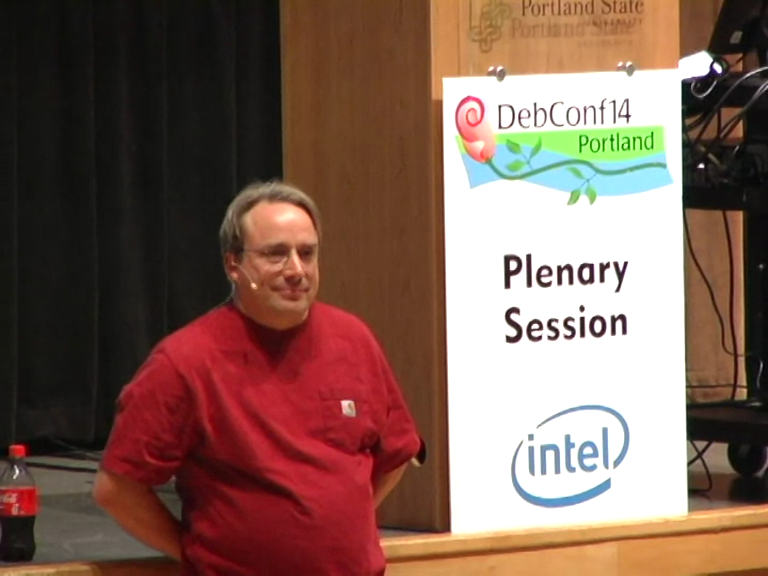
\includegraphics[width=0.7\hsize]{image201409/qa_linus.png}
\end{center}
\caption{セッション名:Q\&A with Linus Torvalds}
\end{figure}


\end{frame}

\begin{frame}{Q\&A with Linus Torvalds}

 \begin{itemize}
   \item Linusさんの関心のほとんどはLinuxカーネル。
   \item Debianを触ったのは1度。installに失敗して以来触ってない。ubuntuも同様。
   \item gccの件や、systemdの件など、なかなか厳しい質問が相次ぐ。
   \item Linusのコミュニティ活動に対する本音(?)が聞ける。
   \item 本セッションの発言の品位改善について会場の女性スタッフにツッコまれる。
 \end{itemize}
等など...

\end{frame}

\begin{frame}{大物ゲストその2}
\center{\LARGE Anonymousの研究家登壇!}

\begin{figure}[H]
\begin{center}
 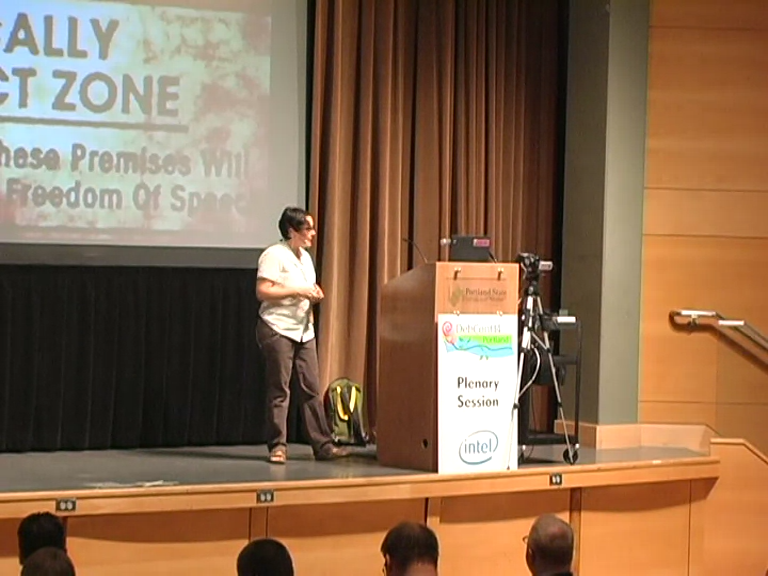
\includegraphics[width=0.6\hsize]{image201409/weapon_geek.png}
\end{center}
\caption{セッション名:Weapons of the Geek}
\end{figure}

 \center{Gabriella Colemanさん}

\end{frame}

\begin{frame}{Weapons of the Geek}

 \begin{itemize}
   \item AnonymousとAnonymousを取り巻く独特のハッカー文化の解説と考察
   \item XENU,Chanology,Scientologyなどの日本人にはなじみの薄いサブカルチャーとAnonymousの関係
   \item Hacktivismについて、Anonymousらの見解。
 \end{itemize}

\end{frame}

\begin{frame}{Debian Project関係}

\center{\LARGE Debian Project関係をいくつか}

\end{frame} 

\begin{frame}{Bit From the DPL}

 まずはこれ。

\begin{figure}[H]
\begin{center}
 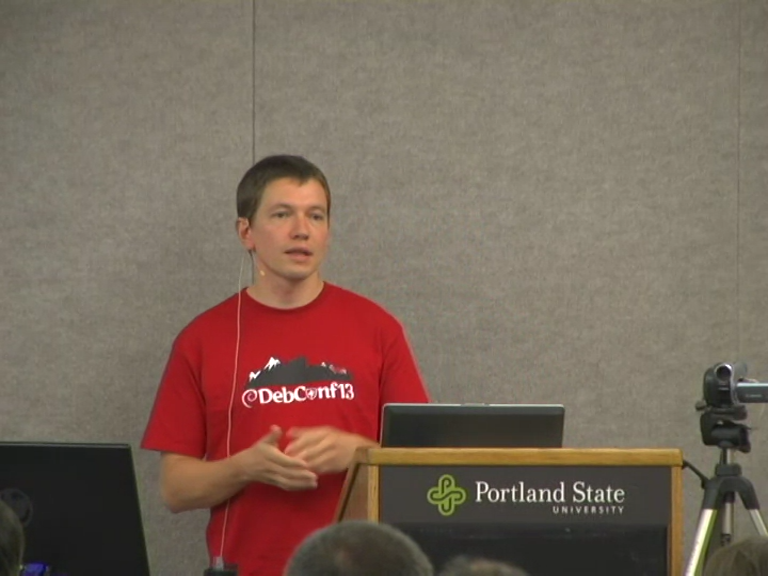
\includegraphics[width=0.6\hsize]{image201409/bit_dpl.png}
\end{center}
\caption{セッション名:Bit From the DPL}
\end{figure}

\end{frame}

\begin{frame}{Bit From the DPL}

 \begin{itemize}
 \item プレゼン資料は、\url{http://blop.info/p/201408-dc14-dpl.pdf}で公開中。
 \item Debian Projectの収支の件の話。現在約2,800万円資産がある。
 \item DebConfの度にお金が増えてしまうので、もうちょっとDebian Projectの活動に使おうとのこと。Debian公式開発者に暗号化用スマートカードを配る、upstreamとのコミュニケーションを活発にする為に使う、mini-DebConfをもっと開催など。
 \end{itemize}

\end{frame}

\begin{frame}{Bit From the DPL}

  Debian ProjectのSWOT解析してみたとのこと。

 \begin{itemize}
   \item 弱み(Weakness) \\
中核部分に関しての完全な人手不足、技術的でない部分への興味のなさと協力者の不足、Debian開発者同士でノウハウの共有化が行われていない場合がある、パッケージ化が難しい、メンター不足やそもそも必要な技術力が高いなどで新参者の開発参加のハードルが非常に高い、upstreamとのコミュニケーションが薄い。
  \end{itemize}

\end{frame}

\begin{frame}{Bit From the DPL}

  SWOT解析続き。

  \begin{itemize}
   \item 脅威(Threats)\\
他のディストリビューションではすでに解決済みのことに対応できていない、Debianの活動をするのに必要なスキル(開発とシステム管理作業など)を習得するような大学のカリキュラムがない、他プログラミング言語が独自で持つパッケージシステムとDebianパッケージの比較をされてしまう。
  \end{itemize}

\end{frame}

\begin{frame}{Jessie bits from the release team}

\begin{figure}[H]
\begin{center}
 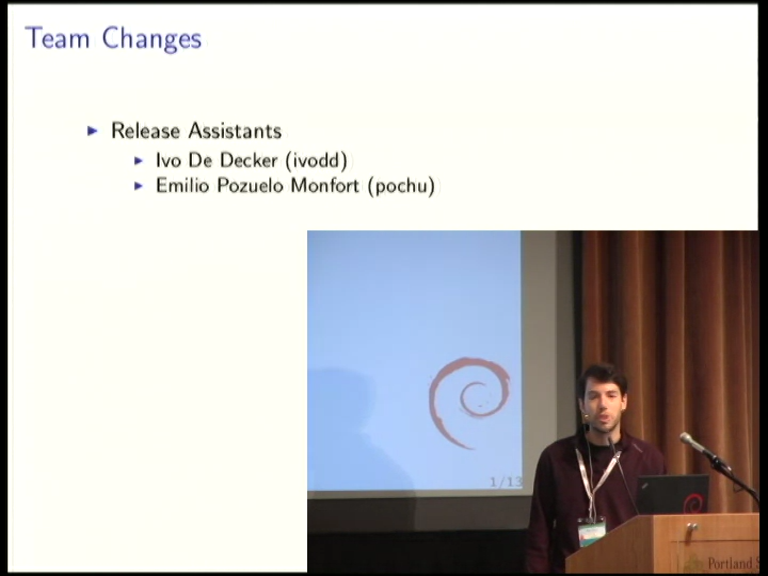
\includegraphics[width=0.6\hsize]{image201409/jessie_release.png}
\end{center}
\caption{セッション名:Jessie bits from the release team}
\end{figure}

\end{frame}

\begin{frame}{Jessie bits from the release team}

 スライドは\url{https://release.debian.org/talks/debconf14/rt-debconf14.pdf}

 内容:
 \begin{itemize}
  \item freezeまでのタイムスケジュールと内容は以下の通り。
    \begin{itemize}
    \item 9/5に新規のtransitionを止める(ライブラリのアップグレードはここで終了)
    \item 10/5より緊急のアップロードを無視しはじめ、testingへの移行に10日かかるようになる。また、セキュリティチームからサポート不可のパッケージの吟味が行われるようになる。
    \item 11/5 Freezeする。
    \end{itemize}
\end{itemize}

\end{frame}

\begin{frame}{Jessie bits from the release team}

\begin{itemize}
  \item 現在のRC bugの残りは450個。2/5以降、testingに移動するのが望ましくないと判断されたパッケージはremoveされる。基本的にどのパッケージもremoveから無事だとは思わないでほしいとのこと。
  \item 今から注意してほしい点として、今からはもう新規のtransitionを提案しないでほしい、Jessieに入れる気の無いパッケージのアップロードは一旦やめてほしい、とにかくインストールテスト(特にUEFI対応のPCを持っている人はできるだけ協力タノムとの事)と、バグを潰してほしいとのことです。
\end{itemize}

\end{frame}

\begin{frame}{日本の参加者の方の発表}

 \center{\LARGE 2名の日本からの参加者の方が発表!}

\end{frame}

\begin{frame}{My PGPGPG key is RSA 2048bit but I put the private key on Gnuk Token}

\begin{figure}[H]
\begin{center}
 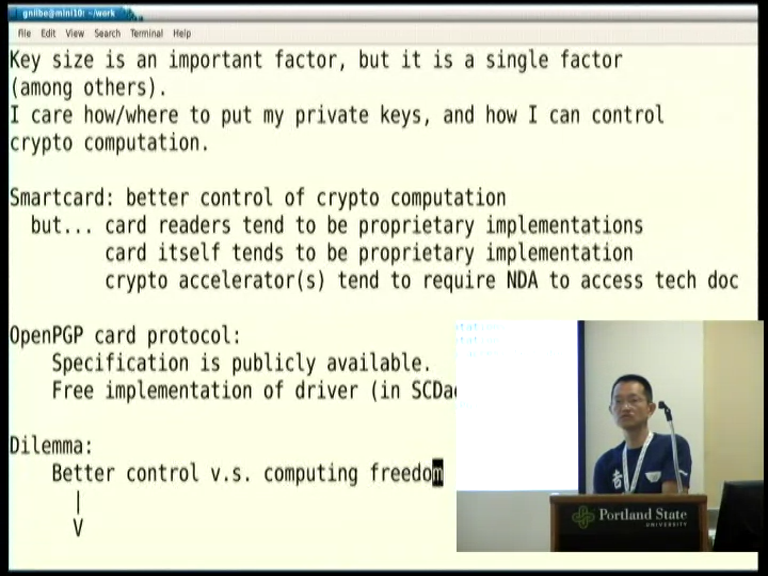
\includegraphics[width=0.6\hsize]{image201409/gnuk.png}
\end{center}
\caption{セッション名:My PGPGPG key is RSA 2048bit but I put the private key on Gnuk Token}
\end{figure}

\end{frame}

\begin{frame}{My PGPGPG key is RSA 2048bit but I put the private key on Gnuk Token}

 スライドは、\url{http://gobby.debian.org/export/debconf14/bof/gnuk}

 \begin{itemize}
 \item 新部さんによるセッション。
 \item 内容はGnuk Tokenの歴史と構造、動作の仕組みについてのセッションです。動作デモもありました。
 \item Gnuk Tokenは、gpgのセキュリティスマートデバイスとして動作できるUSBドングルの事。新部さん開発。このドングルを利用してgpgサインを行えば、暗号処理もドングル内部で行うため秘密鍵を不正に取り出されることもなくセキュアに署名・暗号化が出来る。
 \end{itemize}

\end{frame}

\begin{frame}{My PGPGPG key is RSA 2048bit but I put the private key on Gnuk Token}

 \begin{itemize}
  \item Gnuk Tokenでは、乱数発生機として、未接続の内蔵ADコンバータの1ビット目を使ったとのこと。
  \item Gnuk Tokenは最大3つの鍵を扱えるとのこと。ストア可能なキーサイズは2kbytesはストアできる。
 \item 動作速度として、1.5秒でDebianパッケージのgpgサインが可能。
  \item  途中、ドングル売ってくれとの聴講者の要望。
  \end{itemize}

\end{frame}


\begin{frame}{find \& imporove some bottleneck in Debian project}

\begin{figure}[H]
\begin{center}
 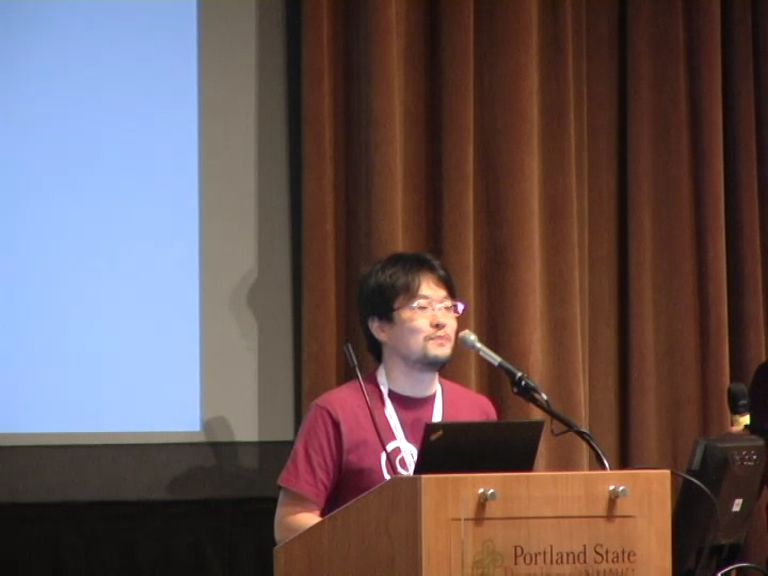
\includegraphics[width=0.6\hsize]{image201409/find_improve.png}
\end{center}
\caption{セッション名:find \& imporove some bottleneck in Debian project}
\end{figure}

\end{frame}

\begin{frame}{find \& imporove some bottleneck in Debian project}

  スライド:\url{http://www.slideshare.net/henrich_d/find-improve-some-bottleneck-in-debian-project\\-debconf14-lt}\\
  動画ファイル名: Lightning\_Talks\_4.webm中 0:43:14あたりで発表。
  
 \begin{itemize}
  \item やまねさんによるライトニングトーク(以下LT)
  \item NEW キューのftpmasterによるチェックに時間がかかる事を解決したいという内容。
 \item review contributorという人を募集し、ftpmasterが現在行っているNEW キューのパッケージチェック作業を、彼ら(複数人)にやらせ、ftpmasterは最終の受け入れのOK/NGのみ出す役割にする。
 \end{itemize}

\end{frame}

\begin{frame}{find \& imporove some bottleneck in Debian project}

 \begin{itemize}
 \item review contributorは、Debian開発者候補としての訓練にも良いし、ftpmasterの作業が過多になってNEW キューが滞るのも解決できて一石二鳥でウマー。
\end{itemize}

\end{frame}

\begin{frame}{その他}

 \center{\LARGE その他発表で興味深いもの}

\end{frame}

\begin{frame}{Debian in the Dark Ages of Free Software}

\begin{figure}[H]
\begin{center}
 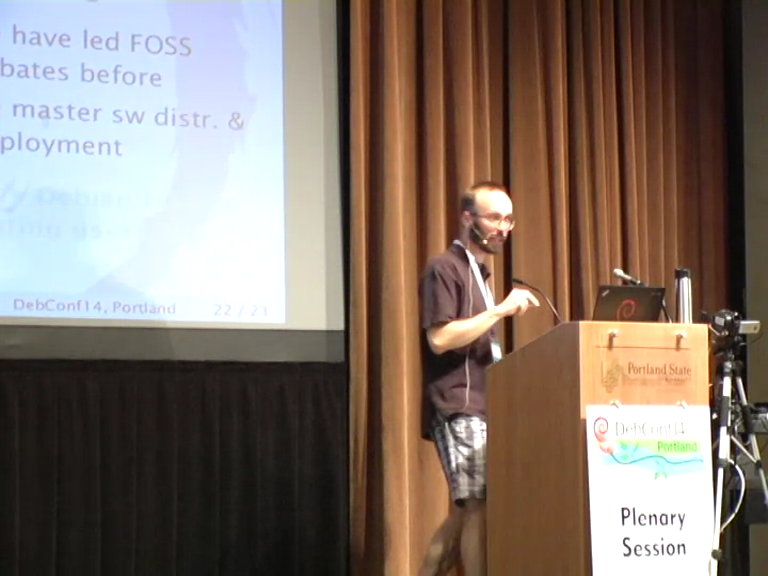
\includegraphics[width=0.6\hsize]{image201409/dark_age.png}
\end{center}
\caption{セッション名:Debian in the Dark Ages of Free Software}
\end{figure}

\end{frame}

\begin{frame}{Debian in the Dark Ages of Free Software}

 \begin{itemize}
 \item  2012年のDPLだったStefano Zacchiroli(以下zack)さんの熱いセッション。
 \item DebianはDFSG Freeなdistoributionを作り普及させたことでは一定の成功を収めた。
 \item OSSも大変身近なものになり、ユーザは、たくさんのソフトウェアについて改変の自由が提供されるようになった。
 \end{itemize}
\end{frame}

\begin{frame}{Debian in the Dark Ages of Free Software}
 \begin{itemize}
  \item しかしながら、これらが成功した一方で、クラウドサービスも進化したため、せっかく勝ち取ったはずのソフトウェアの自由が、クラウドサービスの普及により、結局ユーザの手から取り上げられつつある。
 \item また、自由(Free)Softwareを作るにはFreeの開発ツール/開発環境が究極的には必須であるにもかかわらず、github/Gmailなどユーザからみれば自由でないサービスが益々開発ツール/環境としての地位を強固なものにしている。
 \item このような時代にある事を認識し、これを自由(Free) Softwareの暗黒時代と呼ぼう。
\end{itemize}
\end{frame}

\begin{frame}{Debian in the Dark Ages of Free Software}

{\Large 簡単にいうと、\\
「FOSSが成功を収め、そのおかげでクラウドサービスも爆速で発達したら、
 クラウド技術であるが故にソフトウェアに対するユーザの自由がどう見ても奪われてます。本当にありがとうございました」\\
という状態...orz }
\end{frame}


\begin{frame}{Debian in the Dark Ages of Free Software}

 \begin{itemize}
\item zackさんとしては、解決の良いアイデアが無いので、アイデア募集中とのこと。
\item ライセンスでコントロールしようとか、若い人を教育しようとか、DebianでできたPaaSを作ろうとか。
 \end{itemize}

\end{frame}

\begin{frame}{Welcome talkの一幕}

\begin{figure}[H]
\begin{center}
 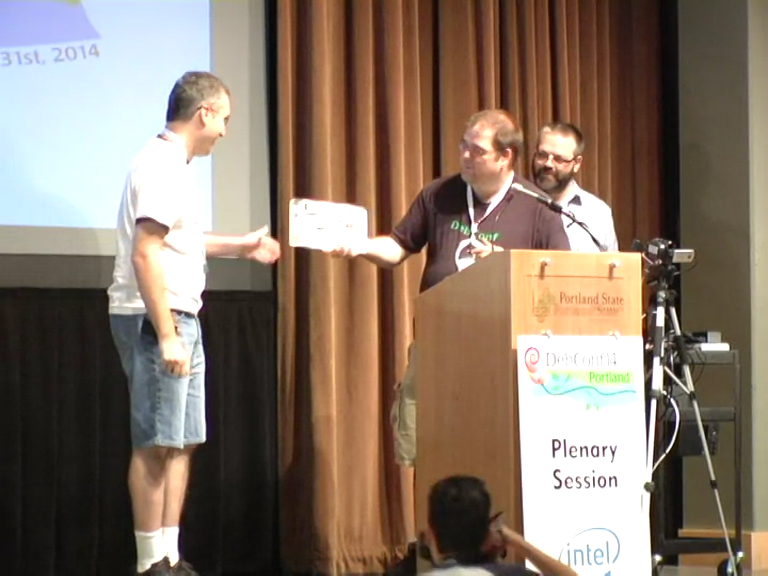
\includegraphics[width=0.6\hsize]{image201409/welcome.png}
\end{center}
\caption{セッション名:Welcome talk}
\end{figure}
 
\end{frame}

\begin{frame}{Welcome talkの一幕}

\begin{itemize}
 \item Welcome talkでの一幕。
 \item steaveおじさんが、russさんを呼んでDebConf14の開催時にスタッフの揉め事を強力なマネジメント力を用いて収めた功績を讃えたシーン。
 \item 贈り物は、今回の揉め事のドタバタをネタにした記念品。
\end{itemize}

\end{frame}

\begin{frame}{Welcome talkの一幕}

 記念品には、アメリカ国防総省の戦争状態のレベルを表すDefcon(Defense Rediness Condition)
\footnote{\url{http://ja.wikipedia.org/wiki/\%E3\%83\%87\%E3\%83\%95\%E3\%82\%B3\%E3\%83\%B3}}のダジャレで、debconという指標が刻まれている。

\end{frame}

\begin{frame}{Welcome talkの一幕}
russさんの読み上げた内容:

\begin{itemize}
\item debcon 5 \\
 メールのやりとりで早期に議論が収まる場合
\item debcon 4 \\
 メールの議論が長期に渡って収まらずredittとか、HNとかにスレッドの内容が投下され、LWNに議論の内容がニュースで投稿されるような事態
\end{itemize}

\end{frame}

\begin{frame}{Welcome talkの一幕}
\begin{itemize}
\item debcon 3 \\
 いわゆるDQNが発生してスレで暴れて議論が荒れ、仕方無いので、ML管理者がDQNをbanするような事態
\item debcon2 \\ 
 例えるとUNが黙ってないようなレベル\footnote{野島注:debianは国際協調プロジェクトだからね!。} UNが行動起こすかの投票まで行われるような事態。つまり議論が苛烈しすぎて戦争レベル。
\item debcon1 \\
 レーザー兵器が衛星に打ち込まれるレベル(要は、議論がもはや収集つかずにカオス状態。)
\end{itemize}
\end{frame}

\begin{frame}{おわりに}

 \center{\LARGE 他にもたくさん面白い発表がありましたが、あとは皆さんで見てね!字幕起こしてね!}

\end{frame}


\section{今後のイベント}
\emtext{今後のイベント}
\begin{frame}{今後のイベント}
\begin{itemize}
 \item 関西エリアDebian勉強会
 \item 東京エリアDebian勉強会 OSC Tokyo/Fall 2014出張編
 \item 2014年10月 東京エリアDebian勉強会 2ndやる?
\end{itemize}
\end{frame}

\section{今日の宴会場所}
\emtext{今日の宴会場所}
\begin{frame}{今日の宴会場所}
未定
\end{frame}

\end{document}

;;; Local Variables: ***
;;; outline-regexp: "\\([ 	]*\\\\\\(documentstyle\\|documentclass\\|emtext\\|section\\|begin{frame}\\)\\*?[ 	]*[[{]\\|[]+\\)" ***
;;; End: ***
